\documentclass[12pt,a4paper,openany]{book}
\usepackage{
      vntex,
      caption,
      graphicx,
      float,
      color,
      amsmath
}
\usepackage[utf8]{inputenc}
%\usepackage[vietnam]{babel}
\usepackage[table,xcdraw]{xcolor}
%%%%%%%%%%%%%%%%%%%%%%%
\usepackage{tikz}
\usepackage{
      tikz-timing,
      circuitikz,
      tikz-qtree
}
      \usetikzlibrary{arrows, shapes.gates.logic.US, calc}
      \tikzstyle{branch}=[fill, shape=circle, minimum size=3pt, inner sep=0pt]
      \tikzset{every tree node/.style={minimum width=2em,draw,circle},
         blank/.style={draw=none},
         edge from parent/.style=
         {draw,edge from parent path={(\tikzparentnode) -- (\tikzchildnode)}},
         level distance=1.5cm}
%%%%%%%%%%%%%%%%%%%%%%%%
\usepackage{scrextend}
\addtokomafont{labelinglabel}{\sffamily}
\usepackage{chngcntr}%đặt lại số
\counterwithin{chapter}{part}%đặt lại số section và section
\renewcommand{\thesection}{\thepart .\arabic{section}}%Loại bỏ chapter

\usepackage{geometry}
      \geometry{%Điều chỉnh giấy cho cả file
      total={170mm,257mm},%Cỡ giấy
      left=15mm,%Lề trái
      right=15mm,%Lề phải
      top=20mm,%Lề trên
      bottom=20mm,%Lề dưới
   }
\usepackage{fancyhdr}
\usepackage{lastpage}
      \pagestyle{fancy}
\renewcommand{\headrulewidth}{0.4pt}%Chỉnh độ cao header
\renewcommand{\footrulewidth}{0.4pt}%Chỉnh độ cao footer
\fancyheadoffset[RE,LO]{0\textwidth}%Để canh cho đúng theo chiều ngang của trang.
\fancyhf{}%Bỏ đi số trang chuẩn
      \lhead{TUT5}
      \rhead{CTDL-GT}
      \rfoot{Page \thepage \hspace{1pt} of \pageref{LastPage}} %Phải dưới, số trang

\begin{document}
%%%%%%%%%%%%%%%%%%%%%%%
%%%%%%%%%%%%%%%%%%%%%%%

\newgeometry{%Chỉnh lại cỡ giấy cho các trang sau. Vì lúc nãy dùng cho trang bìa.
total={170mm,257mm},%Cỡ giấy
left=30mm,%Lề trái
right=15mm,%Lề phải
top=20mm,%Lề trên
bottom=20mm,%Lề dưới
}

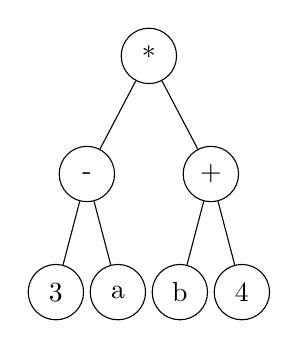
\begin{tikzpicture}
\Tree 
[.* 
      [.- [.3 ] [.a ] ]
      [.+ [.b ] [.4 ] ]
]
\end{tikzpicture}

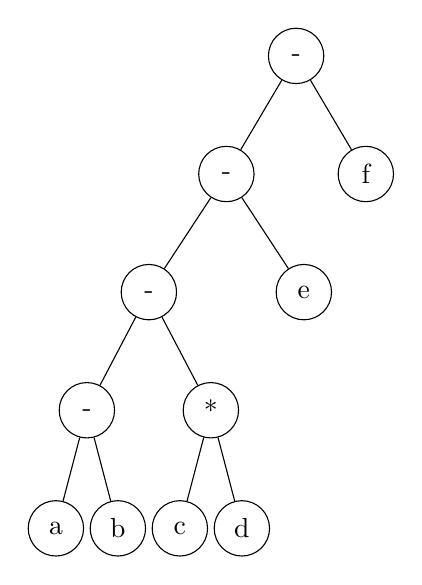
\begin{tikzpicture}
\Tree 
[.-
      [.- 
            [.- 
                  [.- [.a ][.b ]]
                  [.* [.c ][.d ]]
            ]
            [.e ]
      ]
      [.f ]
]
\end{tikzpicture}


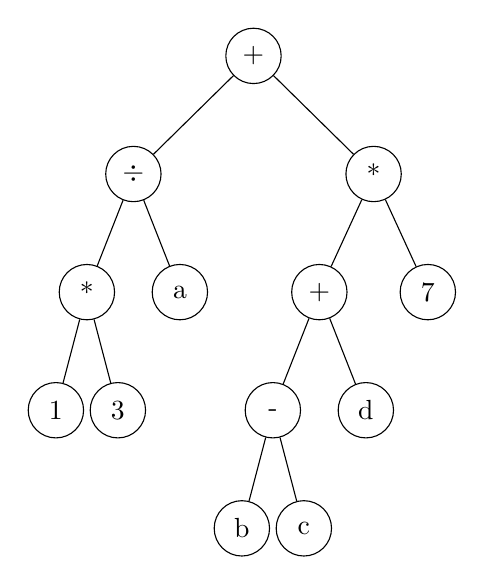
\begin{tikzpicture}
\Tree
[.+
      [.\(\div\)
            [.*
                  [.1 ] [.3 ]
            ]
            [.a ]
      ]
      [.*
            [.+
                  [.-
                        [.b ][.c ]
                  ]
                  [.d ]
            ]
            [.7 ]
      ]
]
\end{tikzpicture}



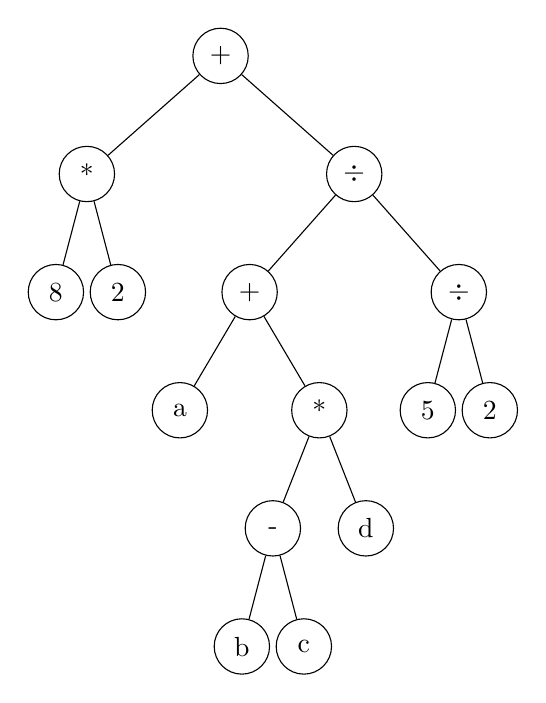
\begin{tikzpicture}
\Tree
[.+
      [.*
            [.8 ][.2 ]
      ]
      [.\(\div\)
            [.+
                  [.a ]
                  [.*
                        [.- 
                              [.b ][.c ]
                        ]
                        [.d ]
                  ]
            ]
            [.\(\div\)
                  [.5 ][.2 ]
            ]
      ]
]
\end{tikzpicture}


\end{document}